\chapter{Timeline}
\label{ch:conclusion}

This chapter provides a timeline of the work for this proposed dissertation. It starts with an overview timeline, summarizing the completed formative work and remaining work on the creativity workshop framework. It concludes with a detailed timeline of the proposed remaining project.

\section{Overview}

This proposed dissertation consists of three projects, two formative design studies followed by the creation of a theoretical framework. We ran the design studies over four years and have been working on the creativity workshop framework for the last two years in parallel with a design study. Here, we briefly describe each project, summarize the role of creativity methods and workshops in it, and list the resulting publications (first author publications are in bold).

\begin{todolist}
    \item[\done] \underline{\emph{{\bf Visual vulnerability analysis}, Sep-2013 -- Dec-'14 (1.5 years)}} --- a design study with defense analysts who were trying to understand the results of ballistic simulations.
    \begin{itemize}
        \item Creativity methods identified shared analysis needs and overcame challenges of working remotely with analysts in a highly secure and large organization
        \item Publications: {\bf design study in Computer Graphics Forum, EuroVis 2015~\cite{Kerzner2015}}; and algorithm in the Journal of Computer Graphics Techniques~\cite{Gribble2014}
    \end{itemize}
    
    \item[\done] \underline{\emph{{\bf Connectome visualization}, May-'15 -- Dec-'16 (1.5 years)}} --- a design study with neuroscientists who were analyzing the circuitry of cells in the retina.
    \begin{itemize}
        \item A creativity workshop established trust, fostered engagement, and exposed shared needs among diverse neuroscientists
        \item Publications: {\bf application/technique in Computer Graphics Forum, EuroVis 2017~\cite{Kerzner2017}}; and biology results in the Journal of Comparative Neurology~\cite{Lauritzen2016}
    \end{itemize}

    \item \underline{\emph{{\bf Visualization creativity workshop framework}, Jun-'15 -- present (2+ years)}} --- an actionable framework that provides theoretical and practical guidance on how to use creativity workshops in design studies.
    \begin{itemize}
        
        \item Analysis of creativity workshops in visualization design, based partly on creativity methods and workshops in the two aforementioned design studies.

        \item Anticipated publication: {\bf theory paper submitted to IEEE Transactions of Visualization and Computer Graphics (IEEE TVCG)}
    \end{itemize}
    
\end{todolist}

A majority of the remaining work involves writing the creativity workshop paper, which we describe in detail next. 

\section{Remaining Work}

We outlined the creativity workshop framework in chapter~\ref{ch:creativity} based on over two years of informal discussions and qualitative data analysis. Here is a detailed timeline of the completed work and proposed remaining work for this project.

\begin{todolist}
 
    \item[\done] \underline{\emph{Jun-'15 -- Jan-'17  (1.5 years)}} --- Discussed creativity workshops with collaborators informally. Attempted to write two papers on the topic, but ultimately decided that the papers were not yet ready for submission.
    
    \item[\done] \underline{\emph{Jan-'17 -- May-'17  (4 months)}} --- Created the current seven stage framework based on in-depth analysis of three workshops and an extensive literature review. 
    
    \item[\done] \underline{\emph{6-Jun-'17 -- 8-Jun-'17  (2 days, on-site in London)}} --- Met with collaborators, agreed on the seven stage framework as a foundation for our paper and outlined answers to questions in chapter~\ref{ch:creativity}.
    
    \item \underline{\emph{8-Jun-'17 -- 15-Aug-'17 (2 months)}} --- Draft answers to the questions outlined in chapter~\ref{ch:creativity} based on qualitative analysis of workshop data and collaborative reflection. Write a draft of the paper based on these answers.
    
    \item \underline{\emph{15-Aug-'17 -- 1-Sep-'17  (2 weeks)}} --- Seek external feedback on the paper and framework from other researchers\footnote{Francesca Samsel (Los Alamos National Lab), members of the Vis Design Lab, members of the giCentre}. Revise the framework based on this feedback.
    
    \item \underline{\emph{1-Sep-'17 -- 30-Sep-'17  (1 month)}} --- Write the final paper and submit to IEEE TVCG.

\end{todolist}

Following the paper submission, we will expand this proposal into a dissertation. Allowing for time to write and edit this dissertation, we hope to defend it by the end of the fall semester, 2017. 

%\begin{figure}
%\centering
% 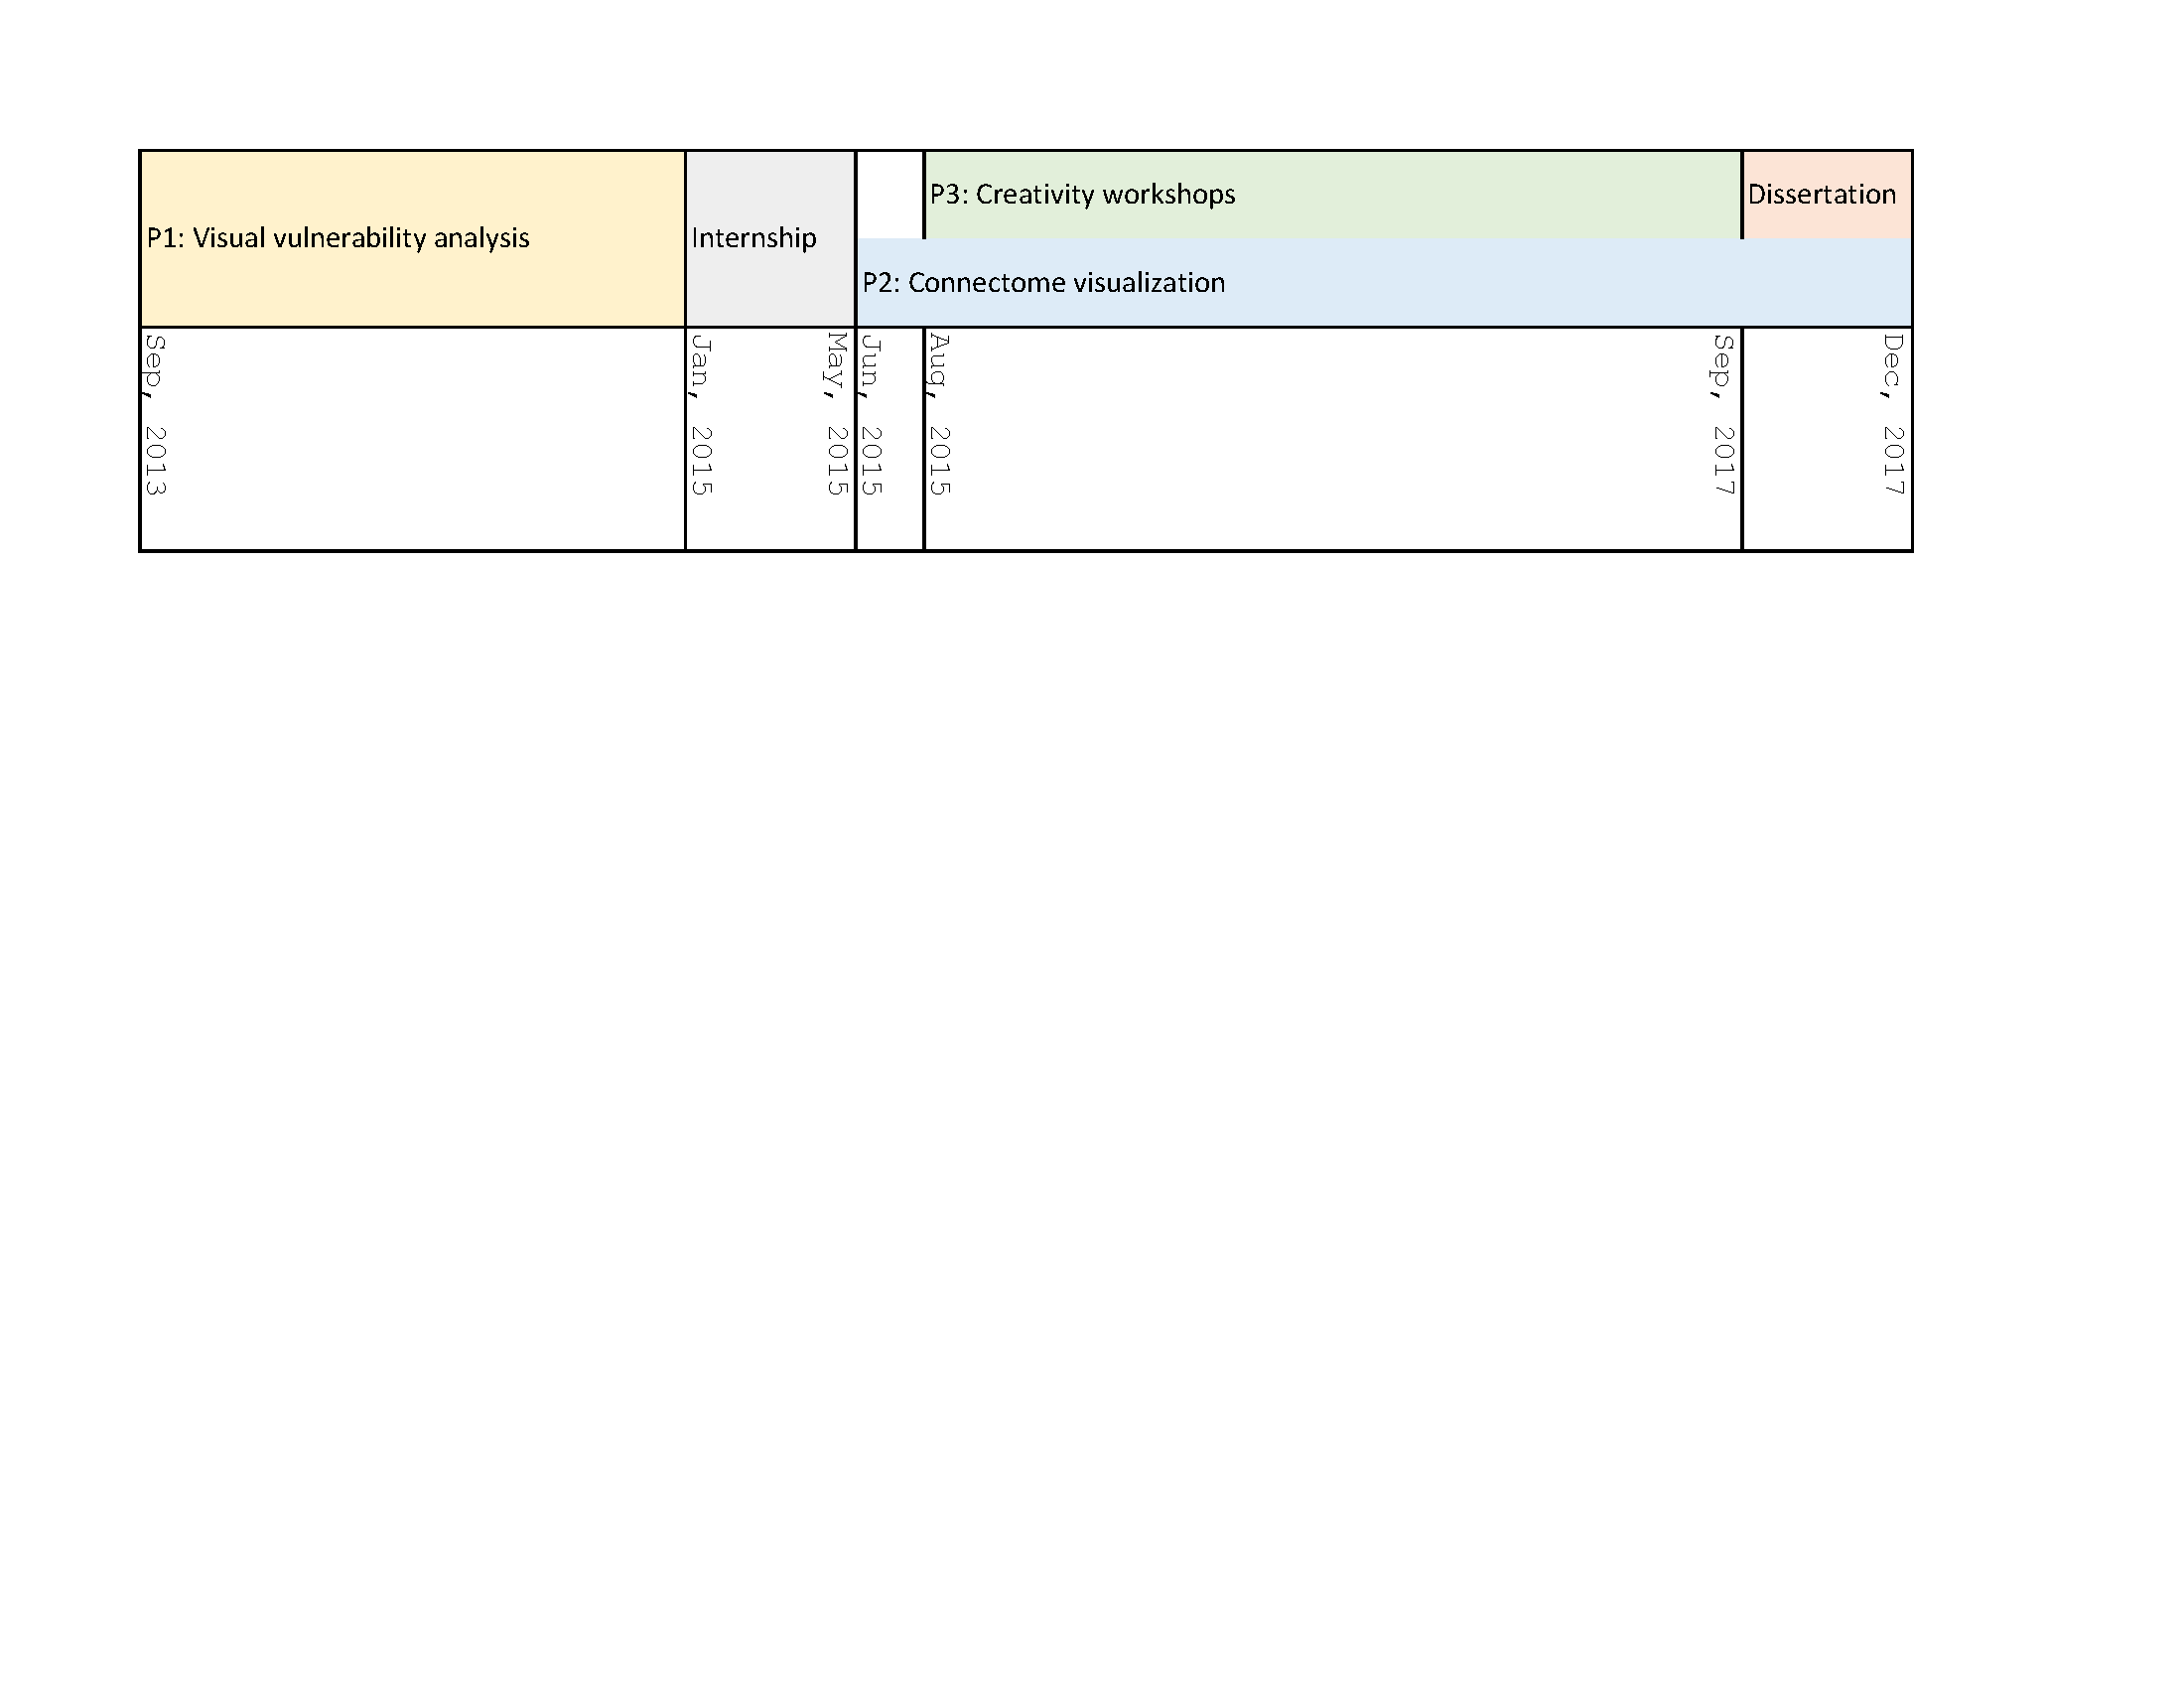
\includegraphics[width=\linewidth,trim={1cm 15cm 2cm 0}]{sources/figures/06_timeline}
  %\caption{Timeline our completed and proposed work spanning the last four years. We propose completing the visualization creativity workshop framework by September, 2017.}
%\label{fig:06_timeline}
%\end{figure}